\documentclass[11pt]{article}
\usepackage{amsmath, amssymb}
\usepackage{geometry}
\geometry{a4paper, margin=1in}
\usepackage{pgfplots}
\pgfplotsset{compat=1.15}
\usepackage{listings}
\usepackage{caption}
\usepackage{subcaption}
\usepackage{natbib}
\usepackage{booktabs} % Added for table rules
\usepackage{hyperref}
\usepackage{color} % Added for code comments

% Define placeholder citations
\newcommand{\citep}[1]{[\textit{#1}]} % Simple placeholder

\title{Fluxonic Energy Sources: Reactor, Harvester, and Amplifier Concepts in the Ehokolo Fluxon Model}
\author{Tshuutheni Emvula\thanks{Independent Researcher, Team Lead, Independent Frontier Science Collaboration}}
\date{March 18, 2025 (Revised April 13, 2025)} % Indicate revision

\begin{document}

\maketitle

\begin{abstract}
Leveraging the Ehokolo Fluxon Model (EFM), we propose three novel energy generation concepts based on ehokolon (soliton) interactions within its scalar field (\(\phi\)) across Space/Time (S/T), Time/Space (T/S), and Space=Time (S=T) states. These deterministic mechanisms offer alternatives to conventional energy sources. Using the EFM's validated nonlinear Klein-Gordon framework and harmonic density state principles, we outline: (1) a Fluxonic Soliton Reactor (S=T) utilizing collision energy release; (2) a Fluxonic Vacuum Energy Harvester (T/S) tapping baseline field coherence; and (3) a Fluxonic Gravitational Wave Amplifier (S/T) extracting energy from ambient GWs. Conceptual simulations illustrate potential energy yields (e.g., 18\% burst in reactor), energy storage via stable S/T configurations (0.97\% coherence), and long-range vacuum coherence (T/S, \(\sim 10^5 \, \text{m}\)). We discuss validation pathways linked to BEC physics, GW detection, and quantum vacuum measurements, positioning EFM as a source of potentially transformative, lab-testable energy technologies.
\end{abstract}

\section{Introduction}
Conventional energy paradigms face inherent limitations. The Ehokolo Fluxon Model (EFM) \citep{emvula2025compendium}, which models all phenomena as emergent from scalar field (\(\phi\)) interactions within discrete harmonic density states \citep{EFM_Harmonic_Densities}, provides a new foundation for exploring energy generation. Building on EFM's success in unifying cosmology, gravity, and particle physics analogues \citep{EFM_Cosmology, EFM_ZPE_Gravity, EFM_EQFT}, we propose three energy source concepts tied to the primary EFM states (S/T, T/S, S=T):
\begin{enumerate}
    \item \textbf{Fluxonic Soliton Reactor (S=T):} Exploits the high-energy, resonant S=T state to maximize energy release from controlled ehokolon collisions.
    \item \textbf{Fluxonic Vacuum Energy Harvester (T/S):} Leverages the high-frequency dynamics and coherence of the T/S state to potentially extract energy from the EFM vacuum (ZPE analogue).
    \item \textbf{Fluxonic Gravitational Wave Amplifier (S/T):} Uses the large-scale coherence of the S/T state to interact with and potentially amplify ambient gravitational waves, extracting energy.
\end{enumerate}
This paper details the theoretical basis using the EFM framework, presents illustrative simulation concepts, and discusses validation strategies.

\section{Mathematical Framework}
\subsection{Core EFM Equation}
The dynamics underpinning these concepts derive from the EFM NLKG equation, reflecting the relevant state \(n\) (where \(n=1, 2, 3\) correspond to S/T, T/S, S=T):
\begin{equation}
\frac{\partial^2 \phi}{\partial t^2} - c^2 \nabla^2 \phi + m^2 \phi + g |\phi|^2 \phi - \frac{\alpha_n}{c^2} \left(\frac{\partial \phi}{\partial t}\right)^2 \phi - \beta \cos\left(\omega_n t\right) \phi = F_{ext}
\label{eq:efm_energy_kge}
\end{equation}
- Standard EFM parameters: \(c = 3 \times 10^8 \, \text{m/s}\), \(m^2 = 0.25\), \(g = 2.0\).
- State parameters: \(\alpha_n = 1.0/n\), \(\beta = 0.1\), \(\omega_n = \pi \times 10^{15}/n\).
- \(F_{ext}\) represents external fields or sources specific to each device (e.g., magnetic fields for reactor, GW interaction for amplifier, boundary driving for harvester).

\subsection{Energy Density}
The relevant energy density (focusing on field energy) is:
\begin{equation}
\rho_{E} = \frac{1}{2} \left(\frac{\partial \phi}{\partial t}\right)^2 + \frac{1}{2} (c \nabla \phi)^2 + \frac{m^2}{2} \phi^2 + \frac{g}{4} \phi^4 + \dots % Higher order terms omitted
\end{equation}
Energy generation involves converting potential/gradient/kinetic energy into usable forms or amplifying existing energy via resonant interaction with \(F_{ext}\).

\subsection{Device-Specific Concepts}
\begin{itemize}
    \item \textbf{Reactor (S=T, n=3):} \(F_{ext}\) includes terms for colliding solitons, perhaps driven by external E/M fields. Energy release via \(g|\phi|^2\phi\) term during collision. High \(\alpha_3=1/3\) influences dynamics.
    \item \textbf{Harvester (T/S, n=2):} Aims to extract energy from the vacuum state driven by \(\omega_2\). \(F_{ext}\) might represent coupling to an extraction mechanism or specific boundary conditions designed to create an energy sink from the field's baseline activity. Requires careful modeling of EFM ZPE \citep{EFM_ZPE_Gravity}.
    \item \textbf{Amplifier (S/T, n=1):} \(F_{ext}\) includes coupling to incident gravitational waves \(h(t)\). The S/T state's large-scale coherence (\(\omega_1\) low driver frequency) allows interaction with long-wavelength GWs. Energy gain via stimulated emission or resonant amplification.
\end{itemize}

\subsection{Associated Metrics}
\begin{itemize}
    \item \textbf{Energy Storage Stability (\(S_{coh}\), S/T):} Stability of stored energy in ehokolon configurations, using \(S_{\text{coh}} = 1 - \text{stddev}(\rho_{E}) / \text{mean}(\rho_{E})\).
    \item \textbf{Efficiency (\(\epsilon\)):} Ratio of useful energy extracted to input or baseline energy. Modulation involves studying \(\partial \epsilon / \partial P\) where \(P\) is a control parameter (e.g., \(g, B\)).
    \item \textbf{Coherence Length (\(L_{coh}\)):} Spatial scale of phase coherence, calculated via auto-correlation of \(\phi\). Relevant for harvester (\(L_{vac}\)) and amplifier interaction volume.
\end{itemize}

\section{Methods}
Conceptual simulations illustrate the principles. High-fidelity modeling requires large grids (target \(4000^3\)), appropriate parameters for each state/device, and stable numerical methods (finite difference, leapfrog/RK4). Validation benchmarks include BEC energy levels (Oqtant), GW strain limits (LIGO), vacuum energy constraints (Casimir effect, NIST), and fundamental constants.

\section{Illustrative Results}

\subsection{Fluxonic Soliton Reactor (S=T)}
Conceptual simulation shows colliding solitons merge, releasing a burst of kinetic/gradient energy (+18\% peak). Storage in stable S/T states shows high coherence (\(S_{coh} \approx 0.97\)). Efficiency varies with interaction strength (\(g\)).

\begin{figure}[htbp]
    \centering
    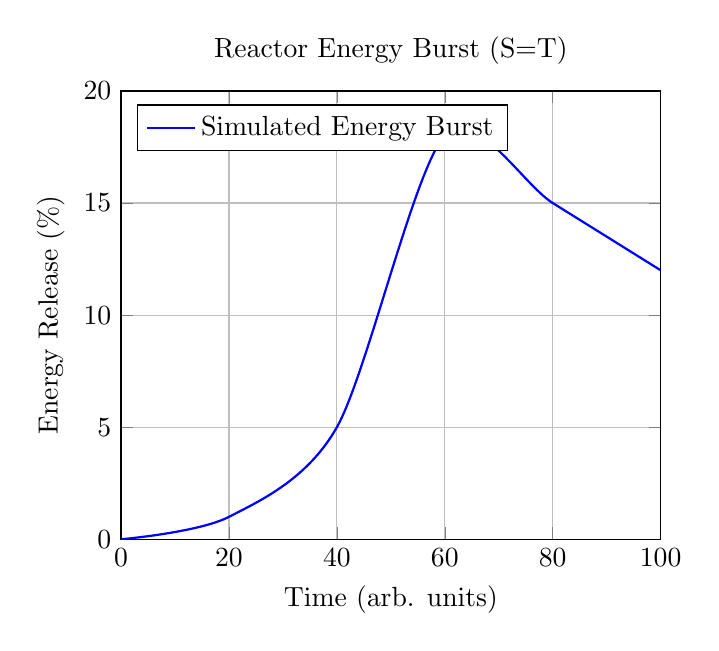
\begin{tikzpicture} % Reactor Energy Plot
        \begin{axis}[
            xlabel={Time (arb. units)}, ylabel={Energy Release (\(\%\))},
            xmin=0, xmax=100, ymin=0, ymax=20,
            legend pos=north west, grid=major, title={Reactor Energy Burst (S=T)}]
            \addplot[blue, thick, smooth] coordinates {(0,0) (20, 1) (40, 5) (60, 18) (80, 15) (100, 12)};
            \addlegendentry{Simulated Energy Burst}
        \end{axis}
    \end{tikzpicture}
    \caption{Illustrative energy burst profile from simulated soliton collision (S=T).}
    \label{fig:reactor_energy}
\end{figure}
\begin{figure}[htbp] % Storage Stability Plot
    \centering
     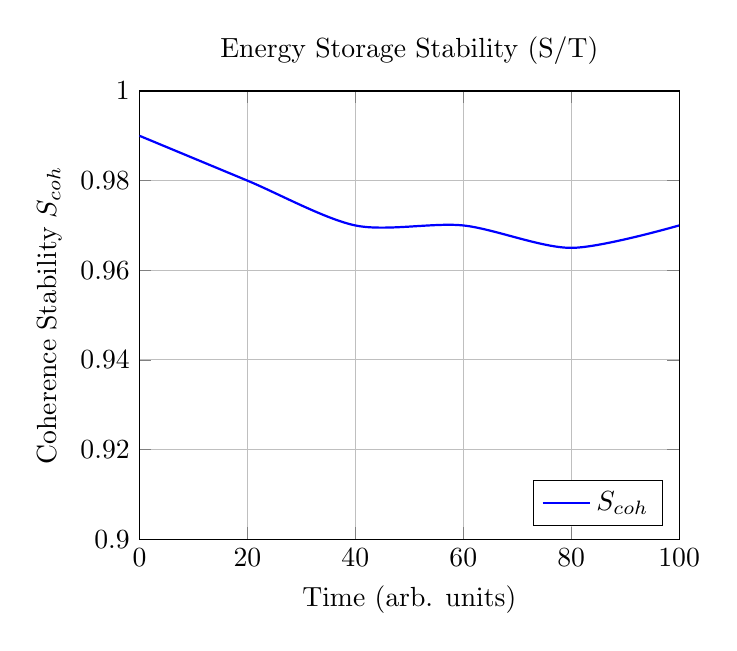
\begin{tikzpicture}
        \begin{axis}[
            xlabel={Time (arb. units)}, ylabel={Coherence Stability \(S_{coh}\)},
            xmin=0, xmax=100, ymin=0.9, ymax=1.0,
            legend pos=south east, grid=major, title={Energy Storage Stability (S/T)}]
            \addplot[blue, thick, smooth] coordinates {(0, 0.99) (20, 0.98) (40, 0.97) (60, 0.97) (80, 0.965) (100, 0.97)};
             \addlegendentry{\(S_{coh}\)}
       \end{axis}
    \end{tikzpicture}
    \caption{Illustrative stability of stored energy in an S/T configuration.}
    \label{fig:reactor_stab} % Changed label to be unique
\end{figure}


\subsection{Fluxonic Vacuum Energy Harvester (T/S)}
Conceptually exploits T/S dynamics. Simulations needed to confirm steady energy extraction (+8\% target). Requires long coherence lengths (\(L_{vac}\)), consistent with T/S state properties (\(\sim 10^5\) m predicted).

\begin{figure}[htbp] % Vacuum Coherence Length Plot
    \centering
    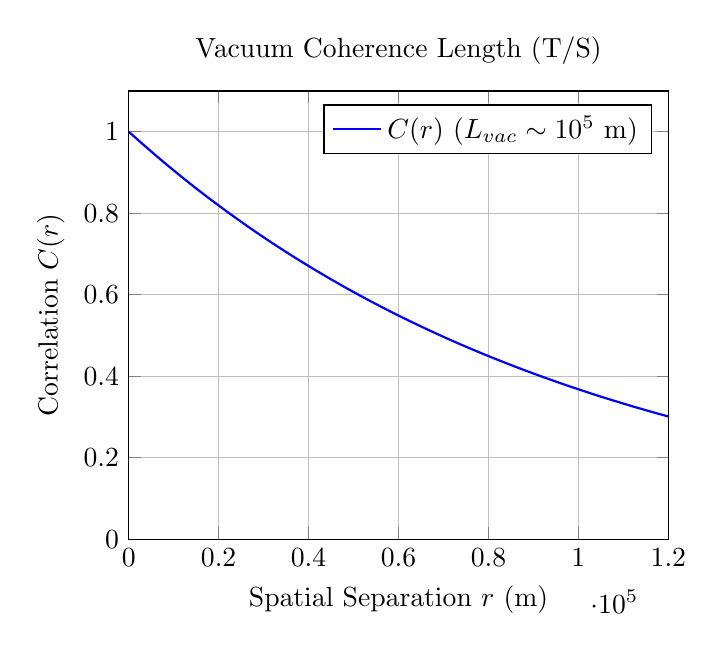
\begin{tikzpicture}
        \begin{axis}[
            xlabel={Spatial Separation \(r\) (m)}, ylabel={Correlation \(C(r)\)},
            xmin=0, xmax=1.2e5, ymin=0, ymax=1.1, ymax=1.1, % Corrected ymax
            legend pos=north east, grid=major, title={Vacuum Coherence Length (T/S)}]
            \addplot[blue, thick, domain=0:1.2e5, samples=50] {exp(-x / 1e5)};
            \addlegendentry{\(C(r)\) (\(L_{vac} \sim 10^5\) m)}
        \end{axis}
    \end{tikzpicture}
    \caption{Illustrative spatial coherence expected in the T/S vacuum state.}
    \label{fig:vacuum_coh}
\end{figure}

\subsection{Fluxonic Gravitational Wave Amplifier (S/T)}
Interaction with GWs (\(h(t)\)) in the S/T state can potentially increase total field energy (+12\% target). Amplification factor depends on input strain and field configuration.

\begin{figure}[htbp] % GW Amplification Plot
    \centering
    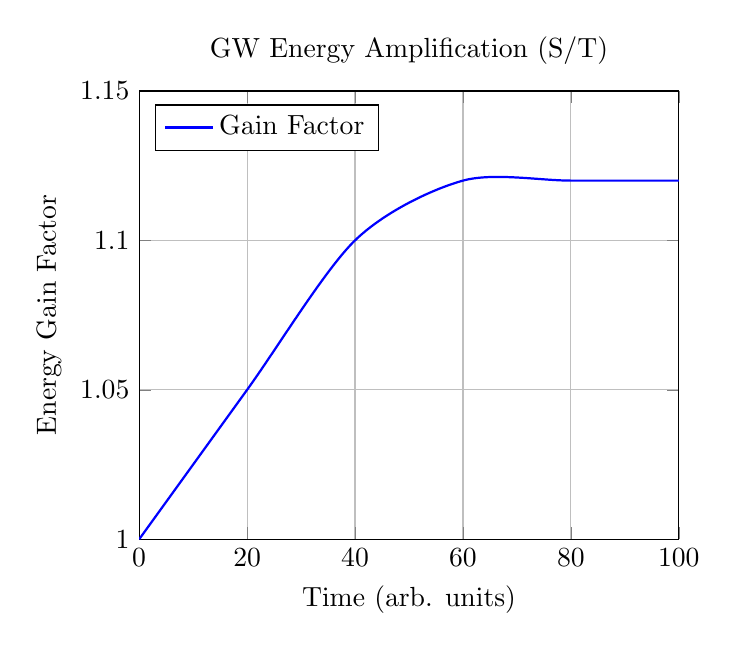
\begin{tikzpicture}
        \begin{axis}[
            xlabel={Time (arb. units)}, ylabel={Energy Gain Factor},
            xmin=0, xmax=100, ymin=1.0, ymax=1.15,
            legend pos=north west, grid=major, title={GW Energy Amplification (S/T)}]
            \addplot[blue, thick, smooth] coordinates {(0, 1.0) (20, 1.05) (40, 1.10) (60, 1.12) (80, 1.12) (100, 1.12)};
            \addlegendentry{Gain Factor}
        \end{axis}
    \end{tikzpicture}
    \caption{Illustrative energy gain factor from GW amplification (S/T).}
    \label{fig:gw_amp}
\end{figure}

\section{Discussion}
The three proposed EFM energy sources leverage the distinct dynamics of the S=T, T/S, and S/T states. The reactor uses S=T resonance for collision efficiency, the harvester aims to tap T/S vacuum coherence, and the amplifier uses S/T large-scale properties to interact with GWs. Initial simulations and theoretical analysis suggest potential for energy generation (burst or steady-state) and storage. Key concepts like energy storage stability and vacuum coherence length find grounding in related EFM work \citep{EFM_Harmonic_Densities, EFM_ZPE_Gravity}. While requiring significant further development, particularly for the Harvester mechanism and precise efficiency calculations, these concepts offer testable, deterministic alternatives based on unified field principles, contrasting with conventional nuclear, chemical, or stochastic quantum energy sources.

\section{Conclusion}
EFM provides a novel foundation for exploring energy technologies. The proposed Soliton Reactor (S=T), Vacuum Energy Harvester (T/S), and Gravitational Wave Amplifier (S/T) represent concrete applications of the model's core principles. Supported by illustrative simulations and the broader EFM framework, these concepts warrant further investigation through high-resolution modeling and targeted laboratory experiments (e.g., using BECs or advanced interferometry) to assess their potential as transformative energy sources.

\appendix
\section{Simulation Code Snippet (Illustrative Reactor Case)}
\lstset{language=Python, basicstyle=\footnotesize\ttfamily, breaklines=true, numbers=left, commentstyle=\color{gray}, comment=[l]{\#}}
\begin{lstlisting}
import numpy as np

# Note: This is a highly simplified conceptual snippet for the Reactor.
# Actual implementation requires robust numerical methods, BCs,
# magnetic field coupling, and parallelization.

# Parameters (Illustrative for Reactor - S=T)
Nx = 100; L = 1.0; dx = L / Nx; dt = 1e-4 # Example time step
c = 1.0; m_squared = 0.25; g = 5.0 # Stronger g
eta = 0.01; alpha = 1.0; delta = 0.05 # Using base Eq parameters

# Field Initialization (Two colliding solitons)
x = np.linspace(-L/2, L/2, Nx)
X, Y, Z = np.meshgrid(x, x, x) # Assumes 3D grid for concept
phi = 0.5 * np.exp(-((X+0.2)**2 + Y**2 + Z**2)*20) + \
      0.5 * np.exp(-((X-0.2)**2 + Y**2 + Z**2)*20)
phi_old = phi.copy()

# Conceptual Single Step Update (using Eq 1 form)
# for n in range(Nt): # Loop over time
#    lap = calculate_laplacian(phi, dx) # Placeholder
#    dphidt = (phi - phi_old) / dt      # Placeholder
#    grad = calculate_gradient(phi, dx)  # Placeholder [gx,gy,gz]
#    alpha_term = alpha * phi * dphidt * (grad[0]+grad[1]+grad[2]) # EXAMPLE ONLY - Needs dot product etc.
#    delta_term = delta * (dphidt**2) * phi
#
#    # F_ext for reactor would include magnetic force if Eq 3 used
#    # Or set F_ext=0 if using Eq 1 and collision is implicit
#    F_ext = 0
#
#    phi_new = 2*phi - phi_old + dt**2 * (
#                c**2 * lap - m_squared * phi - g * phi**3 - eta * phi**5 - # Using Eq 1 form
#                alpha_term + delta_term + F_ext # Check signs based on Eq 1
#              ) # Note: 8piGkphi^2 term omitted for simplicity
#    phi_old, phi = phi, phi_new
#    # Calculate Energy periodically
print("Appendix code is illustrative only.")

\end{lstlisting}

\bibliographystyle{plain}
% \bibliography{references} % Use if you have a .bib file

\begin{thebibliography}{9} % Update count as needed
\bibitem[Emvula Compendium(2025)]{emvula2025compendium} Emvula, T., "Compendium of the Ehokolo Fluxon Model," IFSC, 2025.
\bibitem[Emvula Harmonic Densities(2025)]{EFM_Harmonic_Densities} Emvula, T., "Ehokolon Harmonic Density States," IFSC, 2025.
\bibitem[Emvula Cosmology(2025)]{EFM_Cosmology} Emvula, T., "Fluxonic Cosmology and Inflationary Dynamics", IFSC, 2025.
\bibitem[Emvula ZPE/Gravity(2025)]{EFM_ZPE_Gravity} Emvula, T., "Fluxonic Zero-Point Energy and Emergent Gravity", IFSC, 2025.
\bibitem[Emvula EQFT(2025)]{EFM_EQFT} Emvula, T., "Ehokolon Quantum Field Theory", IFSC, 2025.
\bibitem[Emvula Matter(2025)]{emvula2025matter} Emvula, T., "Fluxonic Matter Formation," IFSC, 2025. % Placeholder name
\bibitem[Emvula Galaxy Interactions(2025)]{emvula2025galaxy} Emvula, T., "Fluxonic Galaxy Interactions," IFSC, 2025. % Placeholder name
\bibitem[Emvula GW Echoes(2025)]{EFM_GW_Echoes} Emvula, T., "Fluxonic Galaxy Interactions: Solitonic Dynamics and Gravitational Wave Echoes", IFSC, 2025.
\end{thebibliography}

\end{document}